\section{Teilaufgabe 28}
\begin{aufgabe}
    Erweitern Sie Ihr Simulink Diagramm mit dieser Vorsteuerung und wählen Sie 
    $F(s) = \frac{1}{K_g}$. Führen Sie ein paar Simulationen durch, beobachten 
    Sie den I-Anteil des Reglers und listen Sie einige Vorteile einer 
    Vorsteuerung auf.
\end{aufgabe}
\begin{figure}[h!]
    \centering
    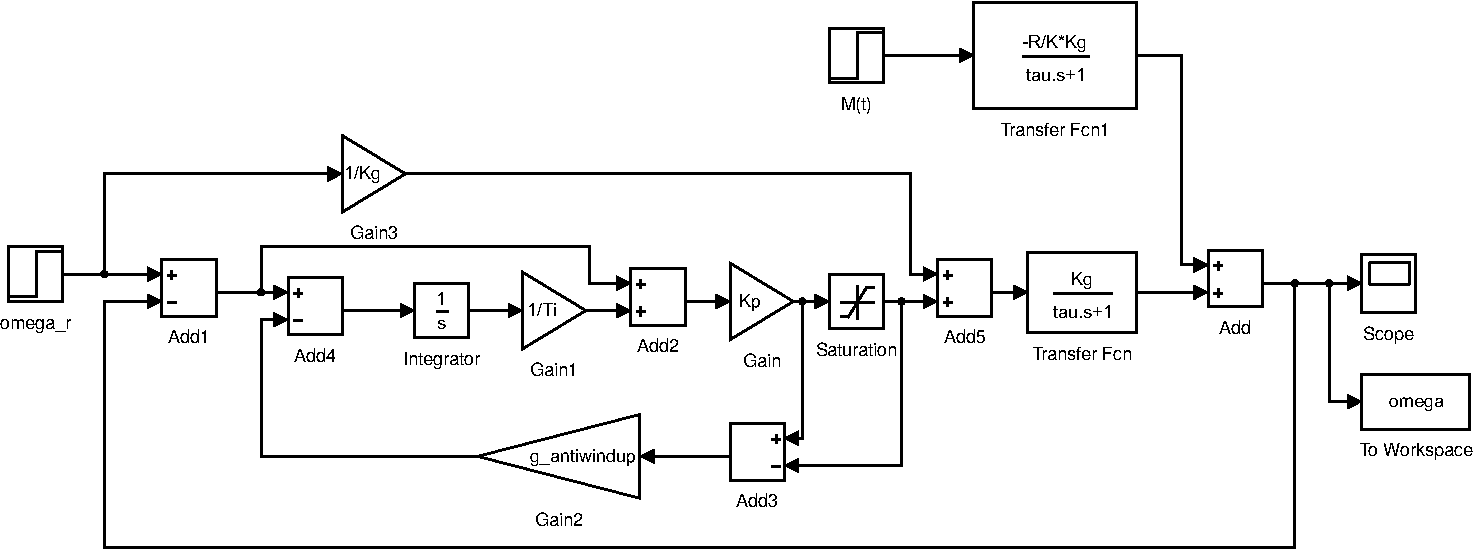
\includegraphics[width=0.6\textwidth]{28/regler_feedforward.pdf}
    \caption{Regler in Simulink}
    \label{fig:28}
\end{figure}
\begin{figure}[h!]
    \centering
    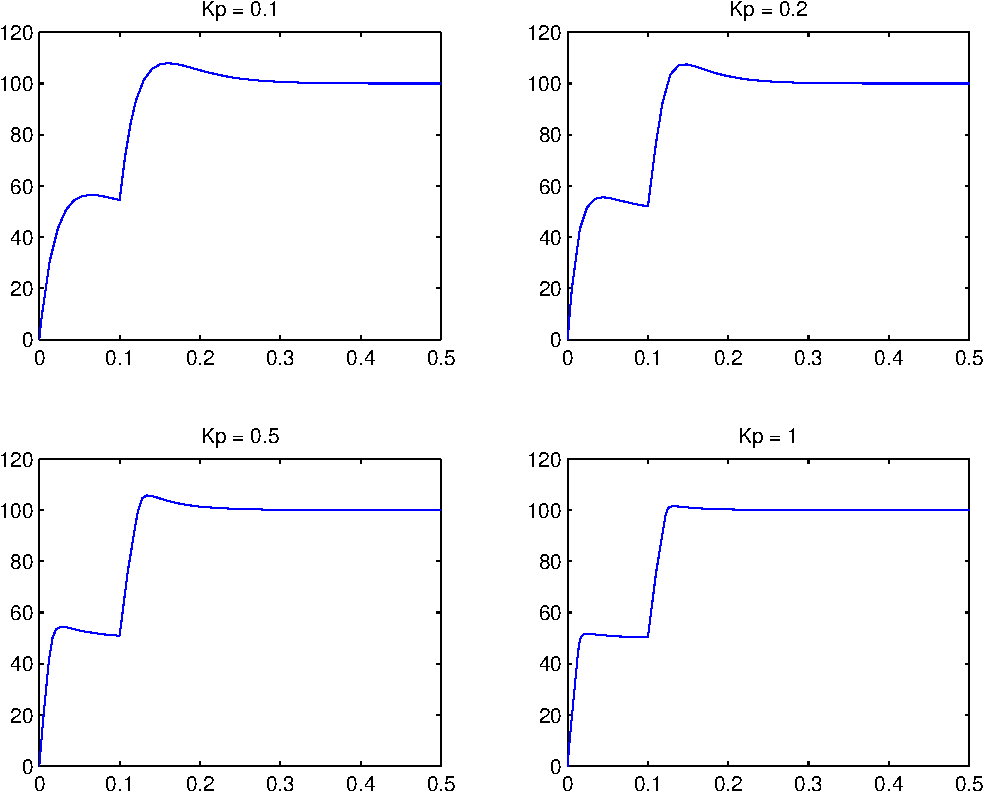
\includegraphics[width=0.6\textwidth]{28/regler_feedforward_plot.pdf}
    \caption{Simulationsergebnis}
    \label{fig:28plot}
\end{figure}
\lstinputlisting{28/regler_feedforward.m}
Der I-Anteil muss im statischen Fall nicht die geasmte Stellgrösse aufbringen. 
Dadurch muss nach einem Sprung der Integrator nicht erst auf den kompletten 
Anteil "'geladen"' werden. \\
$\to$ Der Zielwert wird schneller erreicht. 

